\chapter{Using Markup output with Spreadsheets.}
There are various ways to get SAS output into a spreadsheet.
Each have their advantages and disadvantages.  This chapter
will go over the various tagsets that are good for importing into
spreadsheet programs.

\section{Using CSV}
\index{CSV}
\index{Excel!CSV}
Comma separated values are one of the simplest formats that are
is understood by spreadsheet programs.  The disadvantage is that
there is no formatting, fonts, or colors.  Still CSV files work
very well for many applications.  A CSV file can be connected as
live data to an Excel Template.  This can be a convenient way to
publish Excel spreadsheets to many people.  

The first thing to with the CSV tagset is get help.

\begin{sfvcode}
ODS CSV file='test.csv' options(doc='help');
\end{sfvcode}

The help you get will depend upon which version of the tagset you have.
Amonng the options you will find options to change the delimiter, to
display percentages and currency as numbers,  There are three variables
just to help the tagset know what currency looks like.  You can also
turn titles, notes, procedure titles, and bylines on and off.

By default the csv tagset only displays tables.  Turning on bylines
is a matter of setting the bylines option to yes.

\begin{sfvcode}
ODS CSV file='test.csv' options(delimiter=';' bylines='yes');
\end{sfvcode}


\section{SYLK}
\index{SYLK}
\index{Excel!SYLK}
Symbolic Link format is another simple format for spreadsheet 
programs. SYLK has been around since the days of Visicalc, most 
spreadsheets programs since then have continued to honor this 
file format. SYLK Sylk is slightly better
than CSV because it does contain field formats and data types.

There is a SYLK tagset available on the ODS website at 
http://support.sas.com/rnd/base/topics/odsmarkup/

\section{HTML and Excel}
\index{Excel!HTML}
\index{Excel!CHTML}
\index{Excel!PHTML}
\index{Excel!MSOffice2k}
\index{HTML}
\index{CHTML}
\index{PHTML}
\index{MSOffice2k}
HTML is one of the better ways to import SAS ouput into excel.  But
some tagsets work better than others.  HTML that uses H tags for 
titles, notes and bylines works better than HTML that uses tables
for their formatting.  That makes the HTML4 and HTMLCSS tagsets 
bad choices for importing into Excel.  The Compact HTML, PHTML, and
the MSOffice2k tagsets work the best.  


\section{DDE}
\index{DDE}
\index{Excel!DDE}
There are times when DDE may be the best choice for getting SAS output
into Excel.  DDE can be painful to use because SAS has to connect with
a running Excel session.  A frequent solution to using DDE is to write
a data Step program that writes DDE codes.   A more versatile and reusable
solution is to use the DDE tagset.  Using a tagset to write all the DDE codes
means that anyone can send DDE to Excel with any procedure just by using the 
DDE tagset.

There is a DDE tagset available on the ODS website at 
http://support.sas.com/rnd/base/topics/odsmarkup/


\section{Spreadsheet XML}
\index{SpreadSheetML}
\index{ExcelXP}
\index{Excel!SpreadSheetML}
\index{Excel!ExcelXP}
The ExcelXP tagset generates Spreadsheet XML.  It is probably the best
format for importing SAS ouput into Excel.  SpreadsheetML also works
well with the Open Office.org.  When creating XML with the ExcelXp tagset
it is helpful to know that nameing the file with an xls extension will
cause it load directly into Excel.  Naming the file with an xml extension
will cause Microsoft windows to load the file into Internet explorer as
raw XML.  Open Office.org wants SpreadsheetML files to have an xml extension,
giving it an xls extension will give Open Office.org errors on load. 
 
The very first thing you'll probably want to do with the Excel tagset is
print the help.  Like the other tagsets that take options the Excel tagset
has extensive help.  This is the first place to look for features, options 
and samples.

\begin{sfvcode}
ods tagsets.excelxp file='test.xls' options(doc='help');
\end{sfvcode}


The ExcelXP tagset has over 30 options.  It also uses ODS styles to power
a number of it's features.   The tagattr attribute can be used to rotate
text, and apply Excel formats, and formulas to specific data.

The most basic things to know are that you can control just how the tagset
generates worksheets within your workbook.  The default is one table per worksheet.
But it can be one bygroup per worksheet, or one page, or one procedure.  It can
also be controlled manually within your program.  The worksheets can also be named
however you like.

\begin{sfvcode}

  ods tagsets.excelxp file='multisheet.xls' style=statistical
                      options( sheet_interval='bygroup' );

  proc sort data=sashelp.class out=class;
     by age;
  run;

  proc print data=class;
     by age;
  run;

  ods tagsets.excelxp close;
\end{sfvcode}

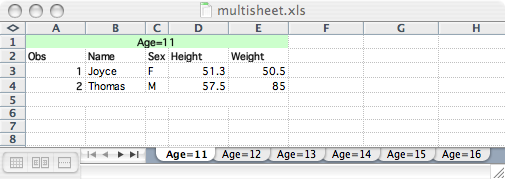
\includegraphics[width=4in]{excelby.png}

SpreadsheetML does have some limitiations.  It does not support graphics.   
The XML it generates can be rather verbose, so the file sizes can be large.

One problem in particular is style over rides as used in proc report, print,
and tabulate.  Over riding style attributes can cause the XML to get very large.
The solution is to create an ODS style and reference those styles by name rather
than just changing the foreground color to red for instance.

The best way to do this sort of thing is to create a style element that you can
use instead of over riding a single attribute of the style.

\begin{sfvcode}
proc template;
     define style styles.mystyle;
            parent=sytles.default;

            style yellow_data from data/
               background = yellow
            ;
      end;
run;

proc print;
   var x /style=yellow_data
\end{sfvcode}

The same end result will be given, except that the style section
of the Excel file will be fairly compact compared to the bloat that
will happen if you do your style over rides like this.


\begin{sfvcode}
proc print;
   var x / style={background=yellow}

\end{sfvcode}


Doing style over rides this way may be more convenient but the 
size of your ExcelXP files can be much larger than anyone would want.


\section{Summary}
When it comes to importing SAS output into spreadsheets there are many choices.
None of them work perfectly.  But some of them work very well.  DDE has been a
popular choice, but using it is somewhat painful.  The excelXP tagset is probably
the best choice for most uses.  The phtml tagset also works very well.


